\chapterimage{}

\chapter*{Conclusion}

\label{chap:conclusion}
\addcontentsline{toc}{chapter}{\nameref{chap:conclusion}}


\fancyhead[LO]{\sffamily\bfseries Conclusion} % Print the nearest section name on the left side of odd pages
\fancyhead[RE]{\sffamily\bfseries Conclusion} % Print the current chapter name on the right side of even pages

The central result of this thesis is the observation of \kmk pairs in the quantum depletion of a weakly-interacting lattice Bose gas. Most of the work I did during my PhD was oriented towards that goal. This measurement was the next step in our task of fully characterizing the correlations across the superfluid-to-Mott insulator transition after the first two works \cite{carcy2019momentum,cayla2020} conducted by the former PhD students Hugo Cayla and Cécile Carcy that focused on the local correlations, respectively deep in the Mott regime and in the superfluid region. 

The first work that I conducted during my PhD is the study the two-body collisions halos \cite{tenart2020two} as a means to complete the previous benchmarking work \cite{cayla2018single} to certify that the measured atomic distribution faithfully represents the in-trap momentum distribution at the level of individual atoms. We devised a simple theoretical model predicting the number of atoms in the collision halos that we validated experimentally by measuring this number for large number of atoms loaded in the lattice. Extrapolating the predictions of the simple model to the low atom numbers usually used in our experiments, we could show that two-body collisions can be safely neglected, proving that our experiment is suited to probe correlations between individual particles. A second work aimed at studying the adiabatic preparation of the gas in the vicinity of the Mott transition \cite{carcy2021}. Led by Cécile Carcy in collaboration with the theoretician Tommaso Roscilde, it has been completed around the middle of my PhD, concluding the series of experiment aiming to prove that our experiment properly simulates the Bose-Hubbard model. In particular, this work showed that it is possible to adiabatically approach the Quantum Critical Point of the superfluid-to-Mott insulator transition at finite entropy, \ie without creating excitations, contrary to the $T=0$ case where this is expected to be impossible. This work then sets the ground for the study of correlations across the superfluid-to-Mott insulator transition that we defined as one of our main point of interest in the introduction to this manuscript.

Our team had attempted before at revealing the pairing mechanism associated to the quantum depletion without success. We identified the low detection efficiency ($\sim 10-15 \%$) as a central issue and thus we decided to implement a two-photon Raman transfer to improve the detection efficiency. Building and testing the Raman transfer was the second main project of my PhD. 

It was more or less at this time that the Covid-19 pandemic hit, forcing us to leave the lab and stay at home. I used this period away from the lab room to develop the algorithm to compute the anomalous correlation function $\gtwo_A$ (to look for the \kmk correlations). I tested and troubleshot this algorithm at first with simulated data and in a second time with the data from the earlier project on the collision halos (in which classical \kmk correlations can be observed in the frame of the center of mass of each halo). 

We started the measurement campaign for the \kmk correlations a few months after the end of first lockdown and were able to observe first experimental signals. We then performed experiments to investigate the role of temperature and of atoms number on the pairing signal and to compare pair correlations with the bunching effect. These measurements provided strong evidences that the observed \kmk correlations were the expected signature of quantum coherences built by atom pairs as a result of interactions. Several features associated with $T=0$ quantum coherences induced by the pairs could be observed and we propose an interpretation in analogy with two-mode squeezed states in Quantum Optics. 

In addition, we observed $\gtwo_A (\bm{0}) \gg \gtwo_N (\bm{0})$, violating the Cauchy-Schwarz inequality, once again signaling the quantum nature of the correlation signal, and finally measured relative number squeezing between modes $\bm{k}$ and $-\bm{k}$. These last two measurements constitute a first step towards demonstrating the presence of entanglement in the many-body equilibrium state of our system. This notably opens the way to characterizing squeezing and entanglement with \textbf{continuous} variables (here the momentum), extending such studies beyond \textbf{discrete} spin variables as mostly done so far.

In a nutshell, we were able to report the first observation of \kmk correlations in an \textbf{at-equilibrium} system, resulting from the interplay between quantum fluctuations and interactions, confirming the 60 years old prediction of Bogoliubov and Lee-Huang-Yang. Interestingly, one of the motivations to observe this signal laid in its conceptual simplicity and the existence of the well-rounded Bogoliubov theory describing it, giving us a general frame to interpret the experimental data. However, the presence of the optical lattice represents an already significant change from the homogeneous Bogoliubov theory and makes theoretical approaches much more complicated and to this day missing. While many of our observations are consistent with Bogoliubov theory, we observed that it notably fails to quantitatively explain the number of detected pairs. This means that our experiment starts to qualify as a quantum simulator as defined in the introduction, even though new theories might emerge in the near future to explain these results as the complexity of the system is still manageable. 

Building up on the quantum simulation aspect, this result is also of great importance for our future experiments as it shows that our experiment is capable of detecting non-local \kmk correlations (we had only observed close-by \kk correlations before), hinting at a possible detection of more complex and hard to predict correlation patterns, notably close the Quantum Critical Point of the Mott transition, that would be a big step towards understanding the physics of strongly interacting many-body systems. This also confirms that we could detect \kmk correlations in Cooper pairs and help understanding the physics of superconductivity with future experiments with fermionic $^3 \rm{He}^*$.

In parallel, I also spent a significant amount of time working on the project of measuring Tan's contact in 1D gases, in collaboration with Hepeng Yao and his supervisor Laurent--Sanchez Palencia from Centre de Physique Théorique at Ecole Polytechnique. This work also falls into the general goal of studying many-body interacting systems with a complementary approach to correlation functions, \ie measuring high momentum tails revealing the presence of contact interactions. We implemented a solution to increase the momentum range of the detector by using a magnetic gradient to shift the entire momentum distribution and access the high momentum region, and were able to observe a $\kmf$ decay on various data sets. While the qualitative evolution of the contact with temperature and interaction strength is consistent with theory, there is a large discrepancy with the QMC calculations that remains to this day unexplained and should be the subject of future experiments. Obtaining an agreement with theory would be of primary importance to show that the momentum density at high $k$ can be used to properly characterize the different regimes and crossovers between them in interacting 1D gases.

\section*{Outlooks}

Our measurements of \kmk correlations have voluntarily left constant the lattice depth. An immediate way of pushing these measurements further (that we have already started working on) is to monitor the pairing while progressively increasing the lattice depth. As $U/J$ increases, and with it the strength of the interactions, we should reach a point at which the Bogoliubov approximation is not valid anymore. It would then be interesting to see how this effect translates to the \kmk correlation signal. As mentioned earlier, we notably expect that more complex correlation patterns may appear as the strength of the interactions increases, effectively involving more than 2 particles. These kind of complex correlations are expected to be particularly important at the Quantum Critical Point of the superfluid-to-Mott insulator transition. A short-mid range prospect would then be to develop new data analysis techniques to measure higher order correlation functions, test them in simple cases like by measuring bosononic bunching with more than 2 particles, and finally use them in experimental data progressively closer to the Quantum Critical Point. As obtaining a good enough signal to noise ratio to measure a $n$-th order correlation function gets increasingly difficult as $n$ increases, we would need to take large amount of data at the Quantum Critical Point. This prospect is particularly exciting as no theory predicts what should happen in terms of momentum space correlations at the Quantum Critical Point, making this measurement a true quantum simulation. 

In addition, our observation of the violation of the Cauchy-Schwarz inequality would be enough to obtain the important result of proving the presence of entanglement in momentum space in many-body equilibrium systems if we were able to measure the correlator  $\langle a^{\dagger}_{\bm k} a_{-\bm k} \rangle$ and show that it is negligible, as in Bogoliubov theory. Improving our experimental setup to have the lattice beams required to perform atomic interferometry and measure this correlator then constitutes another interesting outlook.

Another short term objective is to further investigate the discrepancy between the experimental data and the QMC calculations for the measurement of Tan's contact, notably by taking additional data using the newly added two-photon Raman transfer. We hope that the increased detection efficiency would help us being less sensitive to possible effects of the $m_j=0$ impurities while reducing the number of non-transferred $m_j=1$ atoms. While these atoms are supposed to be prevented from falling on the detector thanks to a strong magnetic gradient kick, we observed that there could be unwanted dynamics such as uncontrolled transfer to the $m_j=0$ state that could perturb our measurement. This measurements might then help us to identify eventual problems in the experiment or in the way that we compare our data to the theory.

Finally, a more long term prospect would be to improve the experimental setup to bring the fermionic isotope of Helium, $^3\He$, to quantum degeneracy. This would open the way to study a whole new kind of physics with the great momentum space resolution of our detector. It would be particularly interesting to study the physics of the BEC-BCS transition and directly measure \kmk correlations in a Cooper pair. To do so, we would first need to identify a usable Feshbach resonance to create the Cooper pairs as there have currently not been a proper investigation of the existence of Feshbach resonance in $^3\He$. 

\renewcommand{\thefigure}{1}
\begin{figure}[h!]
    \centering
    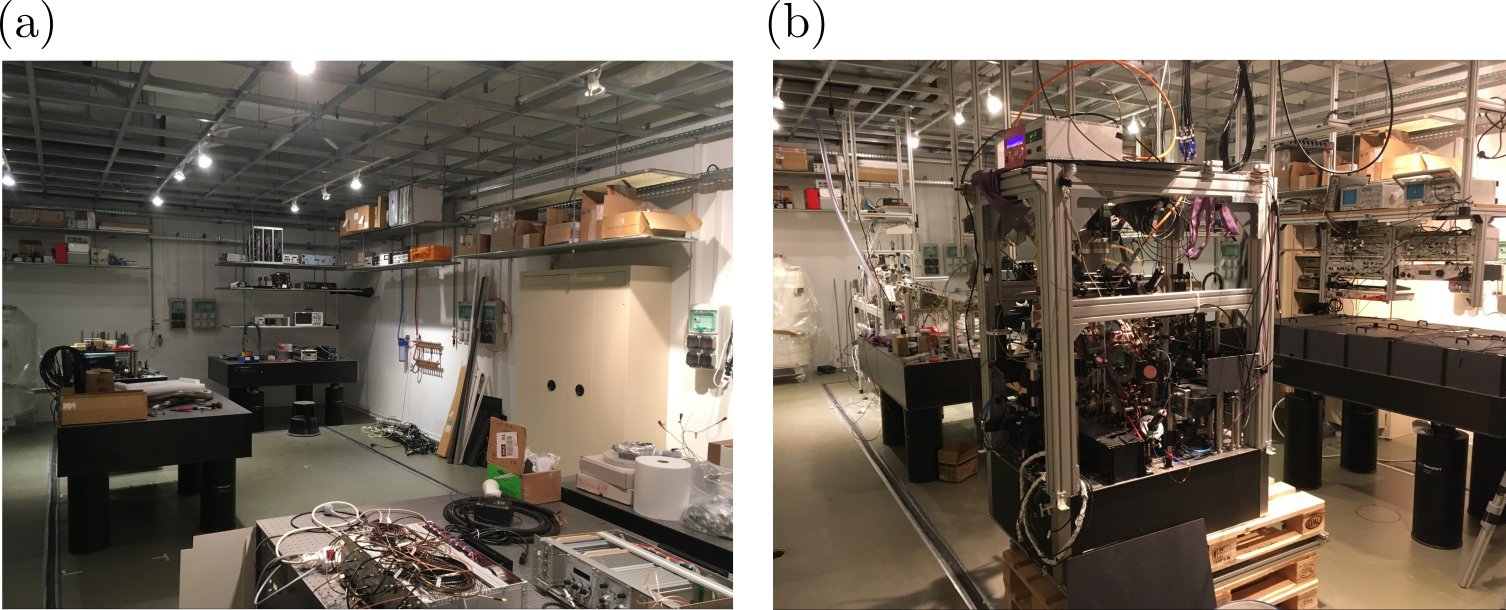
\includegraphics[width=0.95\textwidth]{Fig/Conclusion/before_after.png}
    \caption[The new experiment room]{The new experiment room. (a) Before moving in, with only a few optical tables left by the previous occupants of the room. (b) After moving in.}
    \label{fig:before_after}
\end{figure}

Actually, the lab room in which all the experiments of this thesis were conducted was starting to get packed, and adding the new equipment to cool down a new atomic species would have barely left enough space in the room for a PhD student. This last year, we took a first (but big!) step towards the installation of $^3\He$ in our experiment by moving the entire apparatus to a new bigger room a few steps down the corridor (see Fig.-\ref{fig:before_after}), giving us plenty of additional space. At the moment that I am writing this manuscript, we managed to get the experiment back to its working state and were able to produce BECs and should be able to resume taking data soon. I would like to end this manuscript with one last figure (\ref{fig:SC_moving}) which is of my favorite picture of my time as a PhD student, showing the Helium Lattice team in the perilous process of moving the science chamber to the new room, in which I hope it will serve to make many beautiful experiments in the years to come.



\renewcommand{\thefigure}{2}

\begin{figure}
    \centering
    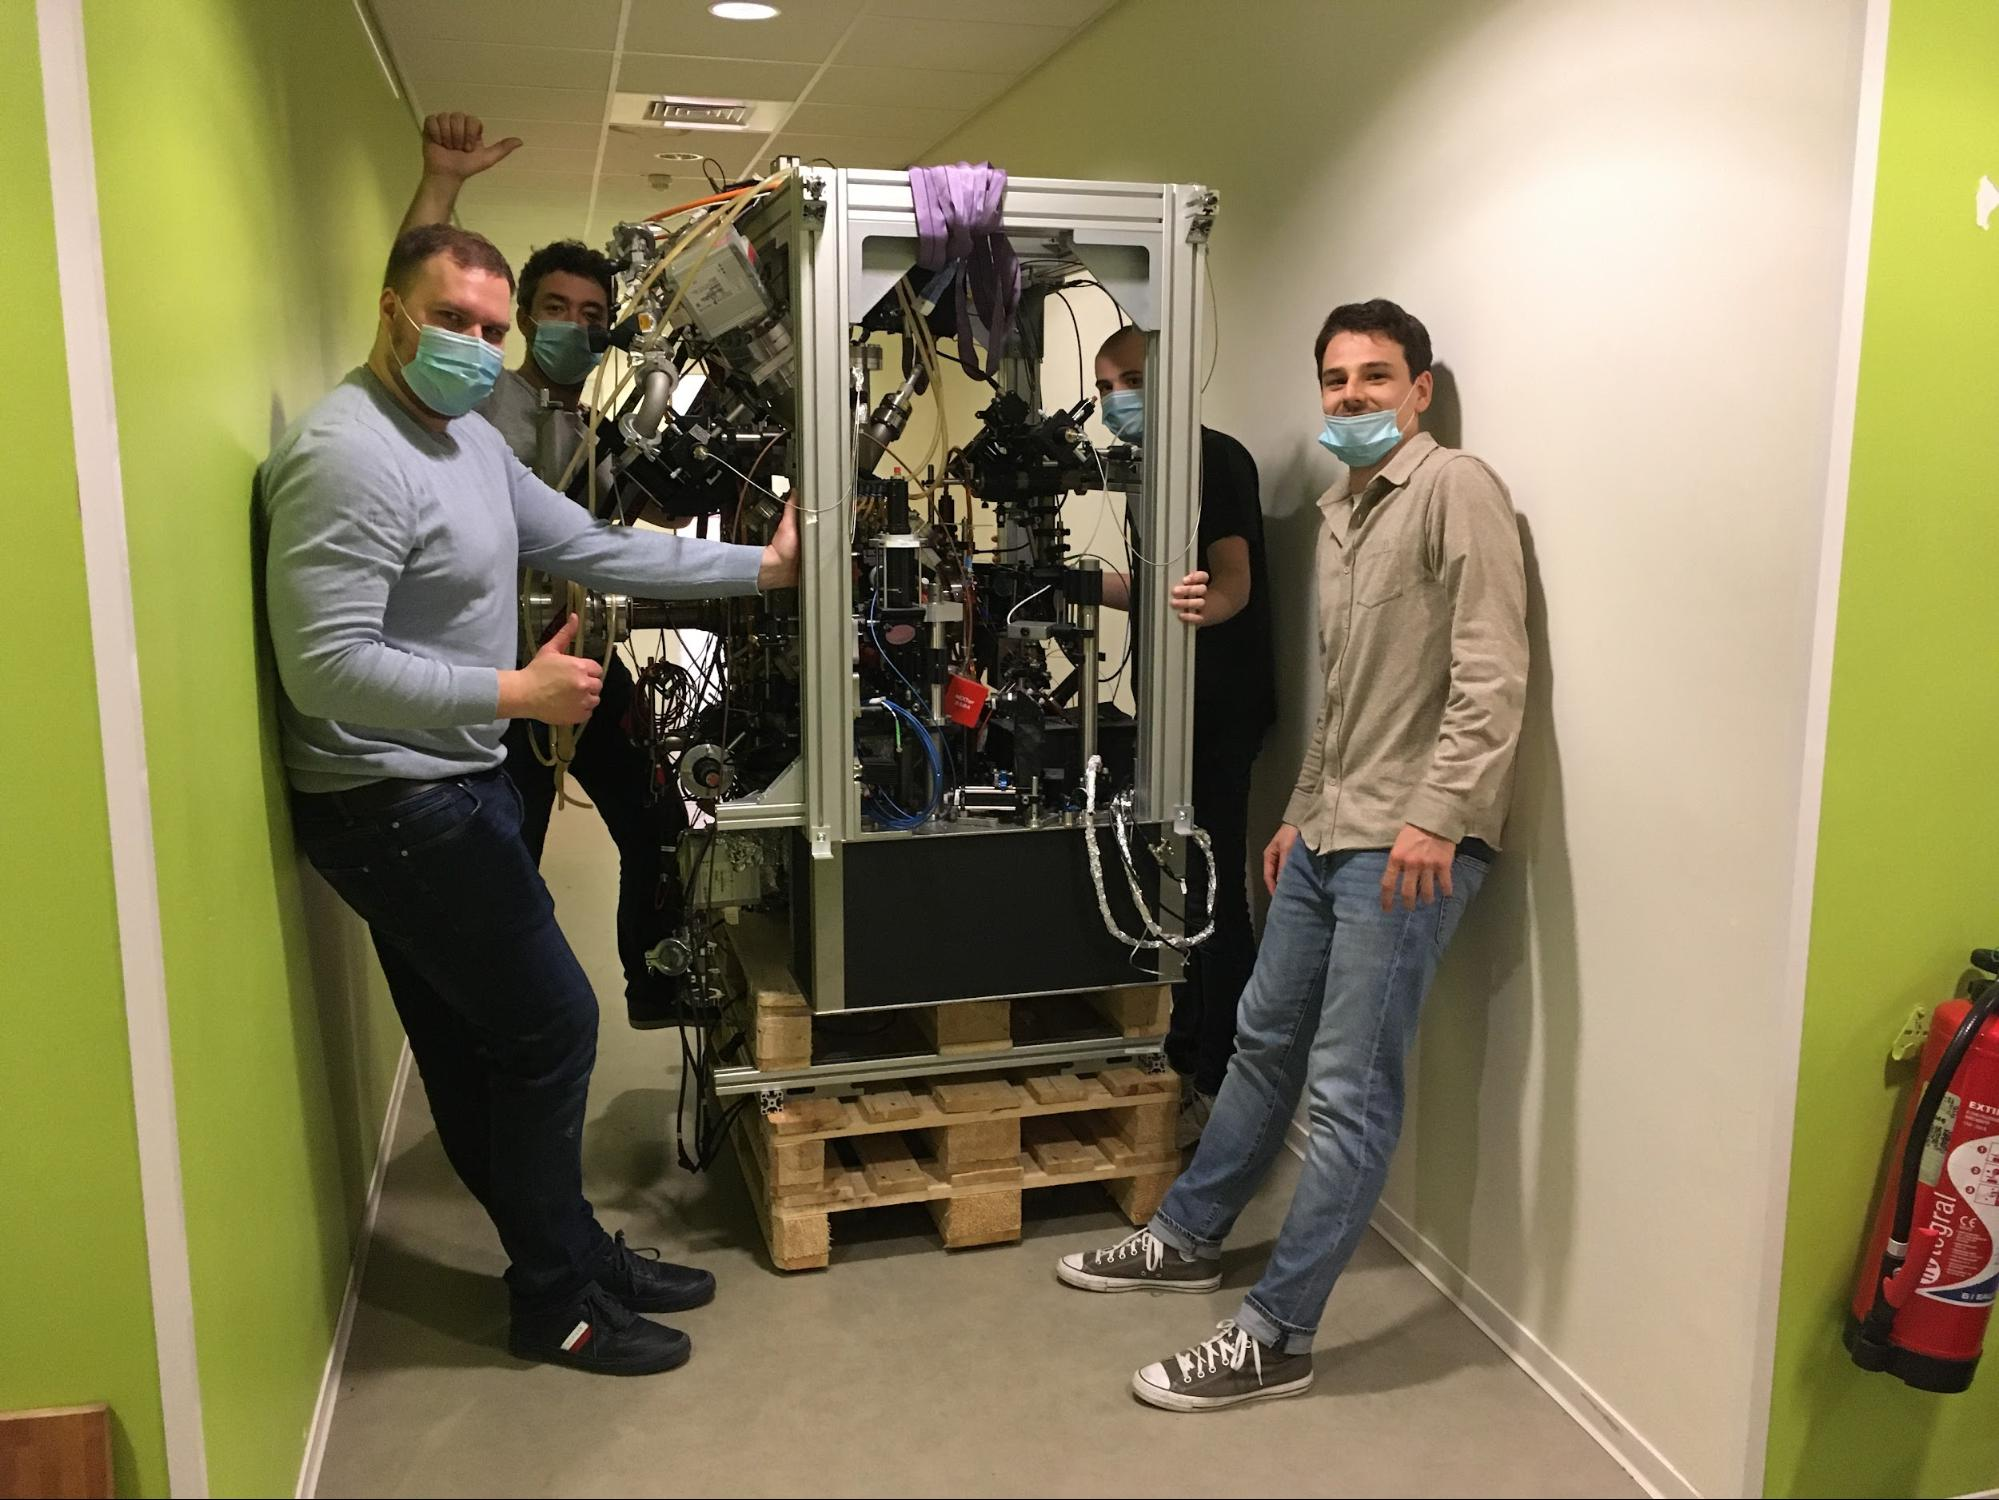
\includegraphics[width=0.8\textwidth]{Fig/Conclusion/SC_moving.jpg}
    \caption{The Helium Lattice team with the Science Chamber, moving from the old room to the new one.}
    \label{fig:SC_moving}
\end{figure}



